\documentclass[border=6pt]{standalone}
\usepackage{tikz}
\usetikzlibrary{arrows.meta,positioning,calc,shapes.geometric,fit,backgrounds,patterns,matrix,decorations.pathreplacing}
\begin{document}
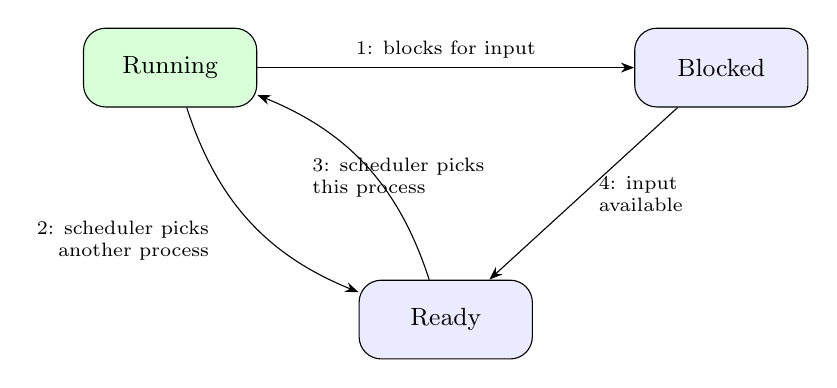
\begin{tikzpicture}[>=Stealth,font=\small]
\tikzstyle{st}=[draw,rounded corners=8pt,minimum width=2.2cm,minimum height=1cm,fill=blue!8]
\node[st,fill=green!15] (r) at (0,0) {Running};
\node[st] (b) at (7,0) {Blocked};
\node[st] (rd) at (3.5,-3.2) {Ready};
\draw[->] (r) -- node[above,font=\scriptsize]{1: blocks for input} (b);
\draw[->] (r) to[bend right=25] (rd);
\draw[->] (rd) to[bend right=25] (r);
\node[font=\scriptsize,align=right] at (-0.6,-2.2) {2: scheduler picks\\ another process};
\node[font=\scriptsize,align=left] at (2.9,-1.4) {3: scheduler picks\\ this process};
\draw[->] (b) -- node[right,font=\scriptsize,align=left,xshift=2pt]{4: input\\ available} (rd);
\end{tikzpicture}
\end{document}
